%; whizzy paragraph -pdf xpdf -latex ./whizzypdfptex.sh
%; whizzy-paragraph "^\\\\begin{frame}"
% latex beamer presentation.
% platex, latex-beamer $B$G%3%s%Q%$%k$9$k$3$H$rA[Dj!#(B 

%     Tokyo Debian Meeting resources
%     Copyright (C) 2009 Junichi Uekawa
%     Copyright (C) 2010 Nobuhiro Iwamatsu

%     This program is free software; you can redistribute it and/or modify
%     it under the terms of the GNU General Public License as published by
%     the Free Software Foundation; either version 2 of the License, or
%     (at your option) any later version.

%     This program is distributed in the hope that it will be useful,
%     but WITHOUT ANY WARRANTY; without even the implied warranty of
%     MERCHANTABILITY or FITNESS FOR A PARTICULAR PURPOSE.  See the
%     GNU General Public License for more details.

%     You should have received a copy of the GNU General Public License
%     along with this program; if not, write to the Free Software
%     Foundation, Inc., 51 Franklin St, Fifth Floor, Boston, MA  02110-1301 USA

\documentclass[cjk,dvipdfm,12pt]{beamer}
\usetheme{Tokyo}
\usepackage{monthlypresentation}
%  preview (shell-command (concat "evince " (replace-regexp-in-string "tex$" "pdf"(buffer-file-name)) "&"))
%  presentation (shell-command (concat "xpdf -fullscreen " (replace-regexp-in-string "tex$" "pdf"(buffer-file-name)) "&"))
%  presentation (shell-command (concat "evince " (replace-regexp-in-string "tex$" "pdf"(buffer-file-name)) "&"))
%  presentation (shell-command (concat "evince " (replace-regexp-in-string "tex$" "pdf"(buffer-file-name)) "&"))

%http://www.naney.org/diki/dk/hyperref.html
%$BF|K\8l(BEUC$B7O4D6-$N;~(B
\AtBeginDvi{\special{pdf:tounicode EUC-UCS2}}
%$B%7%U%H(BJIS$B7O4D6-$N;~(B
%\AtBeginDvi{\special{pdf:tounicode 90ms-RKSJ-UCS2}}

\title{$BEl5~%(%j%"(B Debian $BJY6/2q(B}
\subtitle{$B;qNA(B}
\author{$B>e@n=c0l(B\\IRC nick: dancerj}
\date{2010$BG/(B01$B7n(B23$BF|(B}
\logo{
\includegraphics[width=8cm]{image200607/openlogo-light.eps}}

\begin{document}

\frame{\titlepage{}}

\begin{frame}{Debian$B!!JY6/2qM=Ls%7%9%F%`(B}
 \begin{itemize}
 \item $B%$%Y%s%H$N<g:E<T$,4JJX$KEPO?>pJs$r@_Dj$9$k$3$H$,$G$-$k$3$H!#(B
 \item $B%$%Y%s%H$N<g:E<T$,;vA02]Bj$r@_Dj$7!"2sEz$r4JC1$K<}=8$9$k$3$H$,$G(B
       $B$-$k$3$H!#(B
 \item $B%$%Y%s%H$N<g:E<T$,4JC1$K;22C?M?t$r3NG'$9$k$3$H$,$G$-$k$3$H!#(B
 \item $B%$%Y%s%H$N<g:E<T$,?75,;22C<T$N>pJs$r?WB.$K3NG'$G$-$k$3$H!#(B
 \item $B%$%Y%s%H$N<g:E<T$,;22C<T$KD>@\O"Mm$,$H$l$k<jCJ$,$"$k$3$H!#(B
 \item $B;22C<T$,4JC1$K;vA02]Bj$b$"$o$;$FEPO?$G$-$k$3$H!#(B
 \item $B;22C<T$,%$%Y%s%H;22C$r%-%c%s%;%k$9$kJ}K!$,$"$k$3$H!#(B
 \item $B;22C<T$,;22C$7$F$$$k%$%Y%s%H$rGD0.$9$kJ}K!$,$"$k$3$H!#(B
\end{itemize}
\end{frame}

\begin{frame}{}

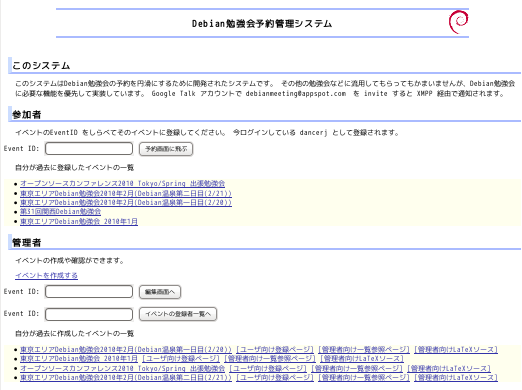
\includegraphics[width=1\hsize]{image201002/debianmeeting-screenshot.png}

\end{frame}

\begin{frame}{Google App Engine for Python}
\begin{itemize}
 \item Python Django $B%Y!<%9$N%&%'%V%"%W%j%1!<%7%g%s%U%l!<%`%o!<%/%[%9%F%#(B
       $B%s%04D6-(B
 \item App Engine $B4D6-$GF0:n$9$k$?$a!"(BDjangos$B$=$N$^$^$G$OF0:n$;$:!"=$@5(B
       $B$,I,MW!#(B
\end{itemize}
\end{frame}

\begin{frame}[containsverbatim]{Google App Engine SDK $B$r%$%s%9%H!<%k(B}
\begin{commandline}
 # apt-get install unzip python$B!!(Bpython-webtest python-yaml
\end{commandline}

$B%=!<%9$O(BDebian$BJY6/2q;qNA$N(B utils/gae $B0J2<!#(B

\end{frame}

\begin{frame}[containsverbatim]{$B%m!<%+%k$G5/F0(B}
\begin{commandline}
$ ../../google_appengine/dev_appserver.py
\end{commandline}
% $ -- for emacs

\url{http://localhost:8080/} $B$G%5!<%S%9Ds6!(B

\end{frame}

\begin{frame}[containsverbatim]{$B%"%C%W%m!<%I(B}

$B%5!<%P$K%"%C%W%m!<%I(B
 \begin{commandline}
$ ../../google_appengine/appcfg.py update
Initiating update.
Email: dancerj@gmail.com
Password for dancerj@gmail.com: 
 \end{commandline}
\url{http://debianmeeting.appspot.com} $B$G%5!<%S%9Ds6!(B
\end{frame}

\begin{frame}[containsverbatim]{$B%F%9%H$N<B9T(B}
 AppEngine $B$N%U%l!<%`%o!<%/$G$O%F%9%HMQ$N%D!<%k$,Ds6!$5$l$F$$$J$$$N$G!"(B
 $B30It%D!<%k$rMxMQ$9$k!#(B
 gaeunit$B$J$I$NA*Br;h$,$"$k!#(B

 python-webtest $B$r3hMQ$7$F%F%9%H$9$k!#(B
 \begin{commandline}
$ PYTHONPATH=../../google_appengine:../../google_appengine/lib/django/ \
 python testSystem.py
 \end{commandline}
\end{frame}


\begin{frame}{$B%G!<%?%Y!<%9$N9=@.(B}
\begin{minipage}{0.4\hsize}
 \begin{itemize}
 \item Event
 \item Attendance
 \item User
 \end{itemize}
\end{minipage}
\begin{minipage}{0.5\hsize}
\begin{itemize}
 \item Event $B$KJ#?t$N(B Attendance $B$,$"$k(B
 \item $B%f!<%6$K$OJ#?t$N(B Attendance $B$,$"$k(B
\end{itemize}
\end{minipage}
\end{frame}


\begin{frame}[containsverbatim]{$B%G!<%?%Y!<%9$N9=@.(B:Event}
$B%$%Y%s%H$r4IM}$9$k(B

\begin{commandline}
 class Event(db.Model):
    eventid = db.StringProperty()
    owner = db.UserProperty() # the creator is the owner
    owners_email = db.StringListProperty() # allow owner emails to be added if possible
    title = db.StringProperty()
    location = db.StringProperty(multiline=True)
    content = db.StringProperty(multiline=True)
    content_url = db.StringProperty()
    prework = db.StringProperty(multiline=True)
    event_date = db.StringProperty()
    timestamp = db.DateTimeProperty(auto_now_add=True)
    capacity = db.IntegerProperty() # the number of possible people attending the meeting
\end{commandline}
\end{frame}

\begin{frame}[containsverbatim]{$B%G!<%?%Y!<%9$N9=@.(B:Attendance}
$B%$%Y%s%H$KBP$7$F$N=P@J$r4IM}$9$k(B

\begin{commandline}
class Attendance(db.Model):
    eventid = db.StringProperty()
    user = db.UserProperty()
    user_realname = db.StringProperty() # keep a cache of last realname entry.
    prework = db.StringProperty(multiline=True) # obsolete, but used in initial version
    prework_text = db.TextProperty() # Used everywhere, populate from prework if available.
    attend = db.BooleanProperty()
    enkai_attend = db.BooleanProperty()
    timestamp = db.DateTimeProperty(auto_now_add=True)
\end{commandline}
\end{frame}

\begin{frame}[containsverbatim]{$B%G!<%?%Y!<%9$N9=@.(B:UserRealName}
$B%f!<%6$NL>A0$r4IM}$9$k(B

\begin{commandline}
class UserRealname(db.Model):
    """Backup of user realname configuration so that user doesn't have to reenter that information."""
    user = db.UserProperty()
    realname = db.StringProperty()
    timestamp = db.DateTimeProperty(auto_now_add=True)
\end{commandline}
\end{frame}

\begin{frame}{$B%=!<%9%D%j!<$N9=@.(B}
\begin{itemize}
 \item \url{debianmeeting.py}: $B$I$N%Z!<%8$,$I$N%3!<%I$r8F$S=P$9$N$+$H$$(B
       $B$&ItJ,$r4IM}$7$F$$$k%3!<%I$G$9!#$"$H!"$I$3$KF~$l$k$N$+LB$C$?%3!<(B
       $B%I$b$3$3$K$"$k$+$b!#(B
 \item \url{admin_event.py}: $B<g:E<T$N%$%Y%s%H$N4IM}4XO"$N%3!<%I$G$9!#(B
 \item \url{user_registration.py}: $B%f!<%6$NEPO?4XO"$N%3!<%I$G$9!#(B
 \item \url{webapp_generic.py}: $B$H$j$"$($:6&DL$N%m%8%C%/$rDj5A$7$F$$$^$9!#(B
       POST $B$H(B GET $B$rF1$8$h$&$K07$&$?$a$N%3!<%I$J$I$,F~$C$F$$$^$9!#(B
 \item \url{schema.py}: $B%G!<%?%9%H%"$N%9%-!<%^$,Dj5A$5$l$F$$$^$9!#(B
 \item \url{send_notification.py}: $B%a!<%kAw?.$H(BXMPP$BAw?.%m%8%C%/$,5-=R$5(B
       $B$l$F$$$^$9!#(B
 \item \url{testSystem.py}: $B%f%K%C%H%F%9%H$G$9!#(B
\end{itemize}
\end{frame}

\begin{frame}{$B%&%'%V%Z!<%8$NA+0\(B}

\includegraphics[width=1\hsize]{image201001/debian-reservation-flow.eps}
 
\end{frame}

\end{document}

;;; Local Variables: ***
;;; outline-regexp: "\\([ 	]*\\\\\\(documentstyle\\|documentclass\\|emtext\\|section\\|begin{frame}\\)\\*?[ 	]*[[{]\\|[]+\\)" ***
;;; End: ***
